%\documentclass[a4paper]{article}
%% Language and font encodings
\documentclass[twocolumn,aps,prl]{revtex4-1}
\usepackage[utf8]{inputenc}
\usepackage[spanish, es-tabla]{babel}
\usepackage[T1]{fontenc}
\usepackage{amsmath}
\usepackage{amssymb}
\usepackage{siunitx}
\usepackage{multirow}
\usepackage{float}
\usepackage{enumitem} % enumerar

\sisetup{math-micro=\text{µ},text-micro=µ}

\usepackage[toc,page]{appendix}

%% Sets page size and margins
\usepackage[a4paper,top=1.5cm,bottom=2cm,left=1.7cm,right=1.7cm,marginparwidth=1.75cm]{geometry}

%% Sets caption text size(its bigger than text)
\usepackage{caption}
\captionsetup[figure]{font=small}
\usepackage{subcaption}

%% Useful packages
\usepackage{svg}
\usepackage{epstopdf}
\usepackage{amsmath}
\usepackage{graphicx}
\usepackage[colorlinks=true, allcolors=blue]{hyperref}

% \newcommand{\nstar}{n^*} 
% \newcommand{\Nstar}{N^*} 

% \newcommand{\N_simulaciones_b}{5000}
\newcommand{\nSimulacionesB}{5000}
\newcommand{\Nsteps}{50}

\newcommand*\sepline{%
  \begin{center}
    \rule[1ex]{.5\textwidth}{.5pt}
  \end{center}}

%%%%%%%%%%%%%%%%%%%%%%%%%%%%%%%%%%%%%%%%%%%%%%%%%%%%%%
%%%%%%%%%%%%%%%%%%%%%%%%%%%%%%%%%%%%%%%%%%%%%%%%%%%%%%

\begin{document}

% ██   ██ ███████  █████  ██████
% ██   ██ ██      ██   ██ ██   ██
% ███████ █████   ███████ ██   ██
% ██   ██ ██      ██   ██ ██   ██
% ██   ██ ███████ ██   ██ ██████

\title{Práctico 3}
\author{M. G. Aramayo}
\affiliation{Matemática de sistemas biológicos, Instituto Balseiro}

% \begin{abstract}
% Mete acá las conclusiones.
% \end{abstract}

\maketitle


% ███████╗██╗  ██╗ ██╗
% ██╔════╝╚██╗██╔╝███║
% █████╗   ╚███╔╝ ╚██║
% ██╔══╝   ██╔██╗  ██║
% ███████╗██╔╝ ██╗ ██║
% ╚══════╝╚═╝  ╚═╝ ╚═╝

\section{Resolución Ej 1:}

\begin{figure}[!ht]
    \centering  
    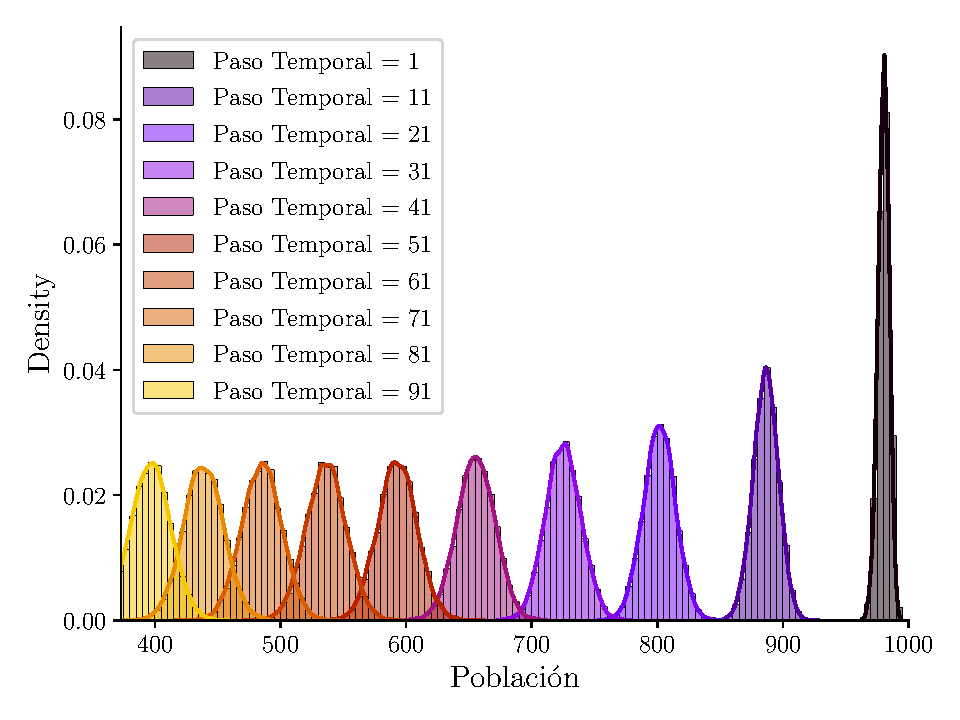
\includegraphics[width=0.5\textwidth]{figuras/ex01-evolucion_temporal.pdf}
    \caption{Evolución en pasos temporales de la distribución de numero de habitantes.}
    \label{fig:ex01-evolucion_temporal} 
\end{figure}

\begin{figure}[!ht]  
    \centering  
    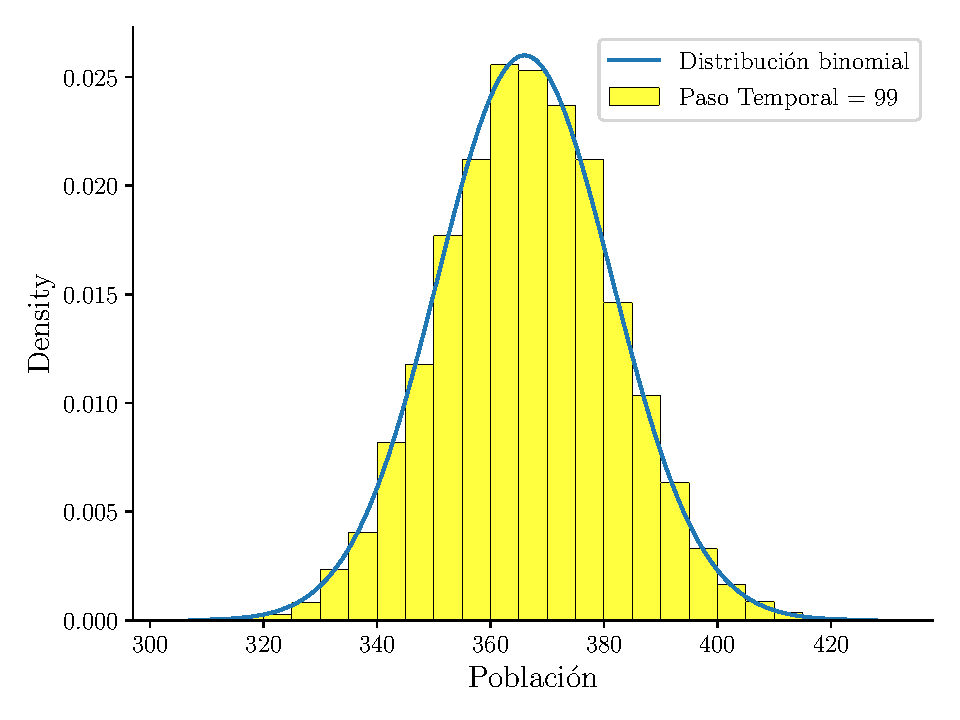
\includegraphics[width=0.5\textwidth]{figuras/ex01-ultima_iteracion.pdf}
    \caption{Comparación entre la densidad obtenida mediante la   simulación y una distribución binomial.}
    \label{fig:ex01-ultima_iteracion}
\end{figure}

% ███████╗██╗  ██╗    ██████╗  
% ██╔════╝╚██╗██╔╝    ╚════██╗
% █████╗   ╚███╔╝      █████╔╝
% ██╔══╝   ██╔██╗     ██╔═══╝ 
% ███████╗██╔╝ ██╗    ███████╗
% ╚══════╝╚═╝  ╚═╝    ╚══════╝

\section{Resolución Ej 2:}

% %%%%%%%%%%%%%%%%%%%%%%%%%%%%%%%%%%%%%%%%%%%%%%%%%%%%%%%%%%%%%%%%
% \sepline
% %%%%%%%%%%%%%%%%%%%%%%%%%%%%%%%%%%%%%%%%%%%%%%%%%%%%%%%%%%%%%%%%

\begin{equation}\label{ec:map01}
  x_{n+1} = a x_n + z_n
\end{equation}

Puede reescribirse como:

\begin{equation}\label{ec:map01-r}
  x_n = a^{n-1} x_0 + \sum_{i=0}^{n-1} a^{n-(1+i)} \ z_i
\end{equation}

\begin{figure}  
  \centering  
  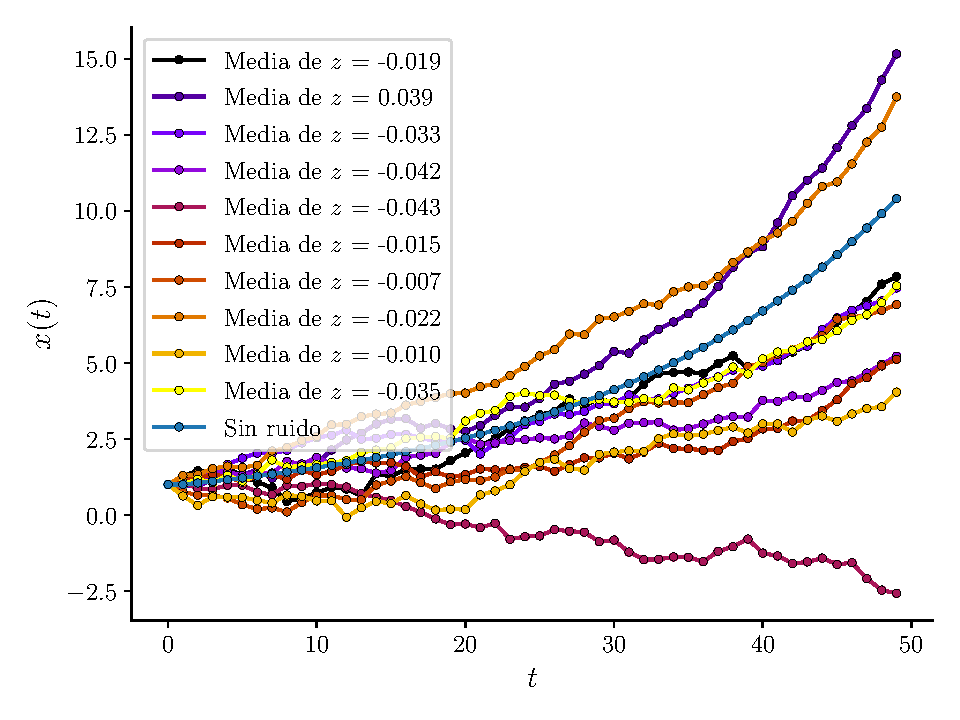
\includegraphics[width=0.5\textwidth]{figuras/ex02-mapeo.pdf}
  \caption{Evolución del mapeo para distintos valores medios de la generación de números aleatorios, para $\Nsteps$ pasos en $t$.}
  \label{fig:ultima_iteracion}
\end{figure}

\begin{figure}  
  \centering  
  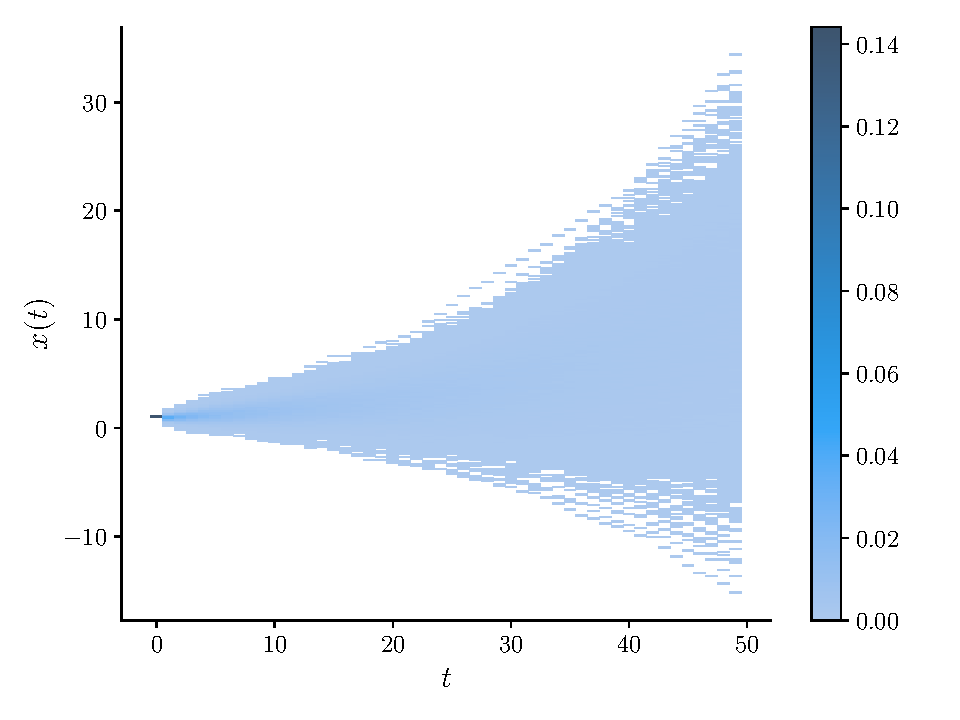
\includegraphics[width=0.5\textwidth]{figuras/ex02-histograma.pdf}
  \caption{$P(x,t)$ densidad de probabilidad (color) de $x$ y $t$ calculada a partir de $\nSimulacionesB$ evaluaciones de $\Nsteps$ pasos en $t$.}
  \label{fig:ultima_iteracion}
\end{figure}

\begin{equation}\label{ec:map02}
  x_{n+1} = (a + z_n) x_n
\end{equation}

Puede reescribirse como:

\begin{equation}\label{ec:map02-r}
  x_n = x_0 \prod_{i=0}^{n-1} (a + z_i)
\end{equation}

\begin{figure}[!ht]  
  \centering  
  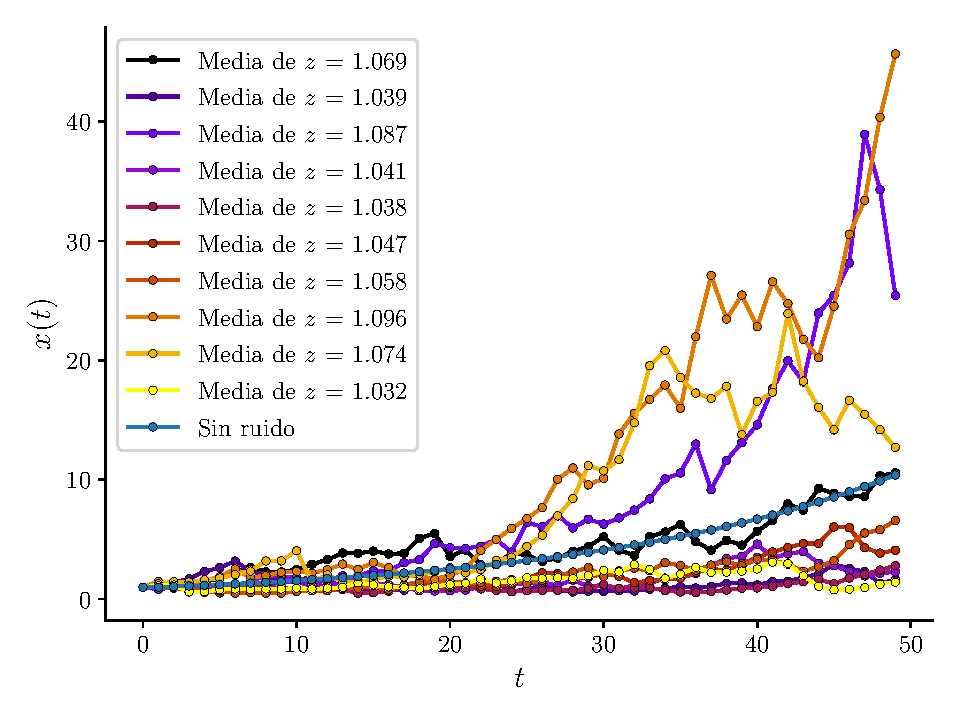
\includegraphics[width=0.5\textwidth]{figuras/ex02-mapeo-02.pdf}
  \caption{$P(x,t)$ densidad de probabilidad (color) de $x$ y $t$ calculada a partir de $\nSimulacionesB$ evaluaciones de $\Nsteps$ pasos en $t$.}
  \label{fig:ultima_iteracion}
\end{figure}

\begin{figure}[!ht]  
  \centering  
  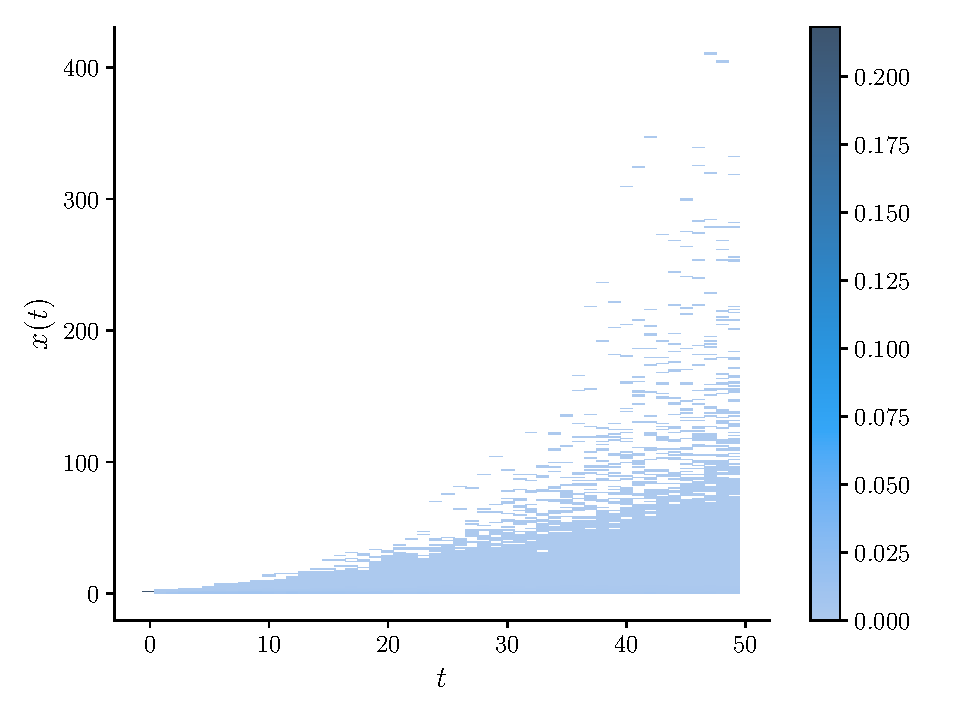
\includegraphics[width=0.5\textwidth]{figuras/ex02-histograma-02.pdf}
  \caption{$P(x,t)$ densidad de probabilidad (color) de $x$ y $t$ calculada a partir de $\nSimulacionesB$ evaluaciones de $\Nsteps$ pasos en $t$.}
  \label{fig:ultima_iteracion}
\end{figure}

% ███████╗██╗  ██╗    ██████╗     
% ██╔════╝╚██╗██╔╝    ╚════██╗    
% █████╗   ╚███╔╝      █████╔╝    
% ██╔══╝   ██╔██╗      ╚═══██╗    
% ███████╗██╔╝ ██╗    ██████╔╝    
% ╚══════╝╚═╝  ╚═╝    ╚═════╝     

% \section{Resolución Ej 3:}

\end{document}
